%%%%%%%%%%%%%%%%%%%%%%%%%%%%%%%%%%%%%%%%%%%%%%%%%%%%%%%%%%%%%%%%%%%%%
%% This is a (brief) model paper using the achemso class
%% The document class accepts keyval options, which should include
%% the target journal and optionally the manuscript type.
%%%%%%%%%%%%%%%%%%%%%%%%%%%%%%%%%%%%%%%%%%%%%%%%%%%%%%%%%%%%%%%%%%%%%
\documentclass[journal=nalefd]{achemso}

%%%%%%%%%%%%%%%%%%%%%%%%%%%%%%%%%%%%%%%%%%%%%%%%%%%%%%%%%%%%%%%%%%%%%
%% Place any additional packages needed here.  Only include packages
%% which are essential, to avoid problems later. Do NOT use any
%% packages which require e-TeX (for example etoolbox): the e-TeX
%% extensions are not currently available on the ACS conversion
%% servers.
%%%%%%%%%%%%%%%%%%%%%%%%%%%%%%%%%%%%%%%%%%%%%%%%%%%%%%%%%%%%%%%%%%%%%
% \usepackage[version=3]{mhchem} % Formula subscripts using \ce{}
\usepackage[T1]{fontenc}       % Use modern font encodings
\usepackage{graphicx,amsmath,mathrsfs,xcolor}
\usepackage{hyperref}        % Remove on submission
\usepackage{todonotes}

%%%%%%%%%%%%%%%%%%%%%%%%%%%%%%%%%%%%%%%%%%%%%%%%%%%%%%%%%%%%%%%%%%%%%
%% If issues arise when submitting your manuscript, you may want to
%% un-comment the next line.  This provides information on the
%% version of every file you have used.
%%%%%%%%%%%%%%%%%%%%%%%%%%%%%%%%%%%%%%%%%%%%%%%%%%%%%%%%%%%%%%%%%%%%%
% \listfiles

%%%%%%%%%%%%%%%%%%%%%%%%%%%%%%%%%%%%%%%%%%%%%%%%%%%%%%%%%%%%%%%%%%%%%
%% Place any additional macros here.  Please use \newcommand* where
%% possible, and avoid layout-changing macros (which are not used
%% when typesetting).
%%%%%%%%%%%%%%%%%%%%%%%%%%%%%%%%%%%%%%%%%%%%%%%%%%%%%%%%%%%%%%%%%%%%%
\newcommand*\subs[1]{_{\text{#1}}} % Text subscription, not available for comma separated
\newcommand*\sups[1]{^{\text{#1}}} %Text superscription
% \newcommand*\change[1]{\textcolor{cyan}{#1}}
\newcommand*\change[1]{{#1}}

%%%%%%%%%%%%%%%%%%%%%%%%%%%%%%%%%%%%%%%%%%%%%%%%%%%%%%%%%%%%%%%%%%%%%
%% Meta-data block
%%
%% Corresponding authors should have an e-mail given after the author
%% name as an \email command. Phone and fax numbers can be given 
%% using \phone and \fax, respectively; this information is optional.
%%
%% The affiliation of authors is given after the authors; each
%% \affiliation command applies to all preceding authors not already
%% assigned an affiliation.
%%
%% The affiliation takes an option argument for the short name.  This
%% will typically be something like "University of Somewhere".
%%
%% The \altaffiliation macro should be used for new address, etc.
%% On the other hand, \alsoaffiliation is used on a per author basis
%% when authors are associated with multiple institutions.
%%%%%%%%%%%%%%%%%%%%%%%%%%%%%%%%%%%%%%%%%%%%%%%%%%%%%%%%%%%%%%%%%%%%%
\author{Tian Tian}
% \affiliation{Institute for Chemical and Bioengineering, ETH Z{\"u}rich,  Vladimir Prelog Weg 1, CH-8093 Z{\"u}rich, Switzerland}
\affiliation{Institute for Chemical and Bioengineering, ETH Z{\"u}rich, Z{\"u}rich 8093, Switzerland}

\author{Peter Rice}
\affiliation{School of Mathematics and Physics, Queen's University Belfast, United Kingdom}
\alsoaffiliation{School of Chemistry and Chemical Engineering, Queen's University Belfast, United Kingdom}

\author{Elton J. G. Santos}
  \email{e.santos@qub.ac.uk}
\affiliation{School of Mathematics and Physics, Queen's University Belfast, United Kingdom}
\alsoaffiliation{School of Chemistry and Chemical Engineering, Queen's University Belfast, United Kingdom}

\author{Chih-Jen Shih}
    \email{chih-jen.shih@chem.ethz.ch}
% \affiliation{Institute for Chemical and Bioengineering, ETH Z{\"u}rich,  Vladimir Prelog Weg 1, CH-8093 Z{\"u}rich, Switzerland}
\affiliation{Institute for Chemical and Bioengineering, ETH Z{\"u}rich, Z{\"u}rich 8093, Switzerland}




%%%%%%%%%%%%%%%%%%%%%%%%%%%%%%%%%%%%%%%%%%%%%%%%%%%%%%%%%%%%%%%%%%%%%
%% The document title should be given as usual. Some journals require
%% a running title from the author: this should be supplied as an
%% optional argument to \title.
%%%%%%%%%%%%%%%%%%%%%%%%%%%%%%%%%%%%%%%%%%%%%%%%%%%%%%%%%%%%%%%%%%%%%
% \title{Penetration of Field Effect in Metal-Oxide-Graphene-Semiconductor Quantum Capacitors}
\title{Multiscale Analysis for Field-Effect Penetration through Two-Dimensional Materials}

%Multiscale Approach for Electric-field Transparency on Two-Dimensional Materials
%Multiscale Approach for Electric-Field Penetration into Two-Dimensional Materials

%Electric-Field Penetration into Two-Dimensional Materials: a Multiscale Approach 

%%%%%%%%%%%%%%%%%%%%%%%%%%%%%%%%%%%%%%%%%%%%%%%%%%%%%%%%%%%%%%%%%%%%%
%% Some journals require a list of abbreviations or keywords to be
%% supplied. These should be set up here, and will be printed after
%% the title and author information, if needed.
%%%%%%%%%%%%%%%%%%%%%%%%%%%%%%%%%%%%%%%%%%%%%%%%%%%%%%%%%%%%%%%%%%%%%
\keywords{Graphene, quantum capacitance, field effect, two-dimensional materials, ab initio calculations, transition metal dichalcogenides}

%%%%%%%%%%%%%%%%%%%%%%%%%%%%%%%%%%%%%%%%%%%%%%%%%%%%%%%%%%%%%%%%%%%%%
%% The manuscript does not need to include \maketitle, which is
%% executed automatically.
%%%%%%%%%%%%%%%%%%%%%%%%%%%%%%%%%%%%%%%%%%%%%%%%%%%%%%%%%%%%%%%%%%%%%
\begin{document}

%%%%%%%%%%%%%%%%%%%%%%%%%%%%%%%%%%%%%%%%%%%%%%%%%%%%%%%%%%%%%%%%%%%%%
%% The "tocentry" environment can be used to create an entry for the
%% graphical table of contents. It is given here as some journals
%% require that it is printed as part of the abstract page. It will
%% be automatically moved as appropriate.
%%%%%%%%%%%%%%%%%%%%%%%%%%%%%%%%%%%%%%%%%%%%%%%%%%%%%%%%%%%%%%%%%%%%%
\begin{tocentry}
\centering
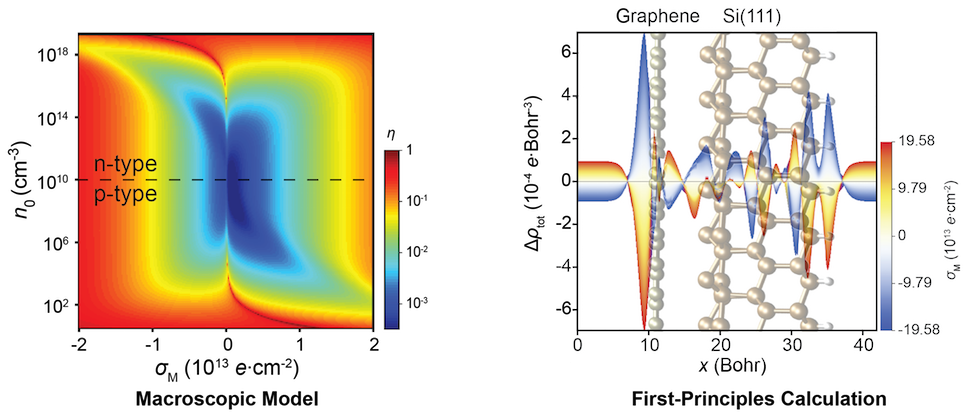
\includegraphics{img/TOC.png}

\end{tocentry}

%%%%%%%%%%%%%%%%%%%%%%%%%%%%%%%%%%%%%%%%%%%%%%%%%%%%%%%%%%%%%%%%%%%%%
%% The abstract environment will automatically gobble the contents
%% if an abstract is not used by the target journal.
%%%%%%%%%%%%%%%%%%%%%%%%%%%%%%%%%%%%%%%%%%%%%%%%%%%%%%%%%%%%%%%%%%%%%
\begin{abstract}
  % We present a theory to model penetration of the field effect through graphene in a metal-oxide-graphene-semiconductor (MOGS) quantum capacitor (QC), including quantifying the degree of ``transparency'' for graphene two-dimensional electron gas (2DEG) to an electric displacement field. 
  % We show that the transparency is determined by the combined effects of graphene quantum capacitance and semiconductor capacitance. The space charge in the semiconductor region is therefore modulated by gating in a nonlinear manner, forming an accumulation or inversion layer at the semiconductor / graphene interface.
  % \textcolor{cyan}{Conclusion of transparency comparison between 2D materials?}
  % Our findings reveal a complete picture of operation modes and design rules for the MOGS QCs.
  Gate-tunable two-dimensional (2D) materials-based quantum capacitors (QCs) and van der Waals heterostructures involve
  tuning transport or optoelectronic characteristics by the field effect. 
  Recent studies have attributed the observed gate-tunable characteristics to the change of 
  the Fermi level in the first 2D layer adjacent to the dielectrics, while the penetration of the 
  field effect through the one-molecule-thick material is often ignored or over-simplified. 
  Here, we present a multiscale theoretical approach that combines first-principles electronic structure calculations 
  and the Poisson-Boltzmann equation methods to model penetration of the field effect 
  through graphene in a metal-oxide-graphene-semiconductor (MOGS) QC, including 
  quantifying the degree of ``transparency'' for graphene two-dimensional electron gas (2DEG) 
  to an electric displacement field.
  We find that the space charge density in the semiconductor layer can be modulated 
  by gating in a nonlinear manner, forming an accumulation or inversion layer at the 
  semiconductor/graphene interface. The degree of transparency is determined by the 
  combined effect of graphene quantum capacitance and the semiconductor capacitance, 
  which allows us to predict the ranking for a variety of monolayer 2D materials according 
  to their transparency to an electric displacement field as 
  follows: 
  \change{graphene > silicene > germanene > WS$\subs{2}$ > WTe$\subs{2}$ > WSe$\subs{2}$ > MoS$\subs{2}$ > phosphorene > MoSe$\subs{2}$ > MoTe$\subs{2}$, 
  }
  when the majority carrier is electron.
  Our findings reveal a general picture of operation modes and 
  design rules for the 2D-materials-based QCs. 
\end{abstract} 

%%%%%%%%%%%%%%%%%%%%%%%%%%%%%%%%%%%%%%%%%%%%%%%%%%%%%%%%%%%%%%%%%%%%%
%% Start the main part of the manuscript here.
%%%%%%%%%%%%%%%%%%%%%%%%%%%%%%%%%%%%%%%%%%%%%%%%%%%%%%%%%%%%%%%%%%%%%
\newpage
The field effect refers to the modulation of the space charge concentration in a semiconductor by applying an electric displacement field \cite{Sze2006Mosfets}.
Over the past few decades, this effect has been utilized to enable a wide range of metal-oxide-semiconductor (MOS) electronics, including the field-effect transistors (FETs) and the floating-gate memory devices \cite{Sze2006Mosfets}.
On the other hand, the two-terminal active electronic components, such as diodes, which consist of semiconductor layers sandwiched between two metallic electrodes, fundamentally prohibit introduction of the field effect due to strong electric-field screening in metal \cite{ehrenreich2001solid}. 
In 1988, Luryi proposed the concept of ``quantum capacitors (QCs)'' and discussed the possibility of using two-dimensional electron gas (2DEG) as one terminal that allows partial penetration of the field effect \cite{Luryi1988Quantum}.
The 2DEG was subsequently realized by trapping electrons in a quantum well \cite{Davies1997Physics} or confining an inversion layer in a metal-oxide-semiconductor (MOS) capacitor\cite{Sze2006Mosfets}.
However, despite great success in demonstration of concept, the 2DEGs are limited in a few materials systems and often require complicated device architecture \cite{stormer1979two}.

Graphene, a zero-bandgap semimetal consisting of a two-dimensional, atomically-thin lattice of sp$^2$-bonded carbon atoms \cite{Novoselov2004Electric}, combines high carrier mobility \cite{Mayorov2011MicrometerScale} and Fermi-energy tunability \cite{Zhang2005Experimental, Das2008Monitoring, Yu2009Tuning}. 
% Recent development in large-area growth and transfer of graphene \cite{bae2010roll} has further shed light on integrating it into different materials systems.
% Therefore, graphene is considered as an ideal candidate of 2DEG \cite{novoselov2012roadmap} to realize the QC devices on a large scale.
Recent development in other two-dimensional semimetals and semiconductors, such as silicene \cite{Aufray2010silicene}, germanene \cite{Davila2014germanene}, 
\change{
  phosphorene (monolayer black phosphorus) \cite{Li2014Phosphorene,Liu2014Phosphorene}
}
and monolayer transition metal dichalcogenides (TMDs) \cite{wang2012electronics}, has further suggested new opportunities in integrating them into different materials systems.
Due to the fact that the thickness of these one-molecule-thick materials is comparable to their Debye screening length, 
they have been considered as the ideal candidates of 2DEG \cite{novoselov2012roadmap} to realize the QC devices on a large scale. 
Very recently, the idea of using graphene 2DEG as one terminal to modulate the characteristics of the two-terminal 
electronic device via gating has been utilized in many graphene-based vertical electronics and 
van der Waals (vdW) heterostructures \cite{geim2013van},
including vertical transistors 
(or barristors) \cite{Yang2012Graphene, yu2013vertically, georgiou2013vertical, Shih2015PartiallyScreened}, solar cells \cite{yu2013highly, britnell2013strong, Regan2012ScreeningEngineered} and light emitting diodes \cite{withers2015light}.
Indeed, most of these devices can be categorized as QCs at some extension.
Nevertheless, most reports have attributed the observed gate-tunable transport 
behavior to the change of graphene's work function, while the penetration of the 
field effect through graphene 2DEG, as well as the effect of the diode bias, are often ignored or over-simplified.
A more complete theoretical picture and analysis are required to elucidate the graphene-based QCs in terms of 
the interplay between the penetration of field effect and the electronic structure of the 2D materials. 

In this letter, we present a mutiscale theoretical approach to model the space charge distribution in a 
metal-oxide-graphene-semiconductor (MOGS) QC giving a quantitative interpretation 
of the field-effect penetration into the device. 
From both macroscopic modeling using Poisson-Boltzmann equation methods
and first-principles {\it ab initio} calculations at different levels of accuracy,
we find that the space charge density in the semiconductor layer can be modulated 
by the field effect through the graphene layer, thereby creating an accumulation or inversion 
layer at the graphene-semiconductor interface. 
Accordingly, the degree of ``transparency'' of the graphene 2DEG to an 
electric displacement field is quantified
and proven to be as a result of the 
combined effect of the graphene quantum 
capacitance, $C\subs{G}$, and the semiconductor capacitance, $C\subs{S}$.
By combining with the density functional theory (DFT) calculations, 
we have used the obtained analytical relations to rank a variety of 2D (e.g. silicene, germanene, 
\change{phosphorene} and 
TMDs)
materials according to their transparency to an electric displacement field. 
Finally, the effect of the bias voltage applied on the semiconductor 
terminal, $V\subs{b}$ is discussed. 
Our analysis show that because the semiconductor capacitance 
increases significantly with $V\subs{b}$, the penetration of the field 
effect in a MOGS QC becomes much less effective beyond a 
certain $V\subs{b}$ range which can guide to optimum design functioning rules.  


Figure \ref{fig:Scheme}a shows an one-dimensional MOGS system comprised of a metal (M) 
electrode, a dielectric oxide (O) layer, a sheet of undoped monolayer graphene (G), 
and a bulk semiconductor (S) layer with the thickness $d\subs{S}$. 
A gate voltage $V\subs{M}$ is applied between the metal and graphene 
terminals to electrostatically induce space charges in graphene and the semiconductor layer. 
An ohmic contact is used on the semiconductor side to apply bias 
voltage $V\subs{b}$ between the semiconductor and graphene terminals. 

\begin{figure}[htbp]
  \includegraphics[width=0.95\linewidth]{img/FIG1.eps}
  \caption{(a) Schematic illustration for the setup of a MOGS QC.  (b) Schematic band diagram of a MOGS QC.}
  \label{fig:Scheme}
\end{figure}

First, the electroneutrality of the entire system suggests:
\begin{equation}
    \sigma\subs{M}+\sigma\subs{G}+\sigma\subs{S}=0
    \label{eqn:charge-balance}
\end{equation}
where $\sigma\subs{M}$ and $\sigma\subs{G}$ and $\sigma\subs{S}$ are the surface charge density in the metal, graphene, and semiconductor terminals, respectively.
The $x$ coordinate is defined as the distance away from the semiconductor/graphene (SG) interface in the semiconductor layer. According to the Gauss's law, $\sigma\subs{S}$ is given by:
\begin{equation}
    \sigma\subs{S} = \int_{0}^{d\subs{S}} \rho(x) dx = -\epsilon\subs{S} \mathscr{E}_0
    \label{eqn:sigma_S}
\end{equation}
where $\rho(x)$ is the space charge density at position $x$ in semiconductor; $\epsilon\subs{S}$ is the dielectric constant of semiconductor, and $\mathscr{E}_0$ is the electric field at the SG interface.
We assume that the electric potential in the semiconductor layer, $\psi(x)$, satisfies the Poisson-Boltzmann equation:
\begin{equation}
    \label{eqn:2nd-poisson}
    \frac{d^2 \psi(x)}{dx^2} = -\frac{e\rho(x)}{\epsilon} = - \frac{e}{\epsilon\subs{S}}[p_0(\text{e}^{-\beta \psi(x)}-1) - n_0(\text{e}^{\beta \psi(x)} -1)]
\end{equation}
where $e$ is the elementary charge, $\beta=e/k\subs{B} T$, $k\subs{B}$ is the Boltzmann constant, $T$ is temperature and $n_0$, $p_0$ are the equilibrium densities of electron and hole in bulk semiconductor, respectively.
Considering the limit that the Debye length in the semiconductor layer $\lambda_D\approx\sqrt{\dfrac{\epsilon\subs{S} k\subs{B} T}{e^2 N\subs{D}}}$ (where $N\subs{D}$ is the dopant density) is much smaller than $d_S$, the boundary conditions $\psi(0)=\psi_0$, $\psi(\infty)=0$ and $\psi'(\infty)=0$ are used for eq \ref{eqn:2nd-poisson}, where $\psi_0$ is the electric potential at the SG interface.
By integrating eq \ref{eqn:2nd-poisson} with respect to $x$, one can determine the semiconductor space charge density $\sigma\subs{S}$ as a function of $\psi_0$ as follows:
\begin{equation}
    %%%%
    % Can be split into  lines if using double column
    %%%%
    \label{eqn:sigma_S_exact}
    \begin{aligned}
    \sigma\subs{S}(\psi_0) = &-\epsilon\subs{S} \mathrm{sign}(\psi_0)\sqrt{\frac{2e}{\beta \epsilon\subs{S}}} \sqrt{p_0(\text{e}^{-\beta\psi_0} + \beta \psi_0 -1) + n_0(\text{e}^{\beta\psi_0} - \beta \psi_0 -1) }
    \end{aligned}
\end{equation}

In order to determine the electric potential at the SG interface, $\psi_0$, the Schottky-Mott rule, which assumes that the vacuum levels for graphene and semiconductor at the interface are aligned, is employed.
Note that this assumption holds when the interface states at the SG interface are negligible  \cite{Xu2011Inducing, Hill1998Molecular}.
% We only consider inorganic semiconductor for this model, since for the interface between graphene and organic semiconductor the assumption of the vacuum level alignment does not hold \cite{Hill1998Molecular}.
It follows that:
\begin{equation}
  \label{eqn:Shottky-Mott}
    \psi_0 = \frac{E_{\mathrm C,\infty} - E_{\mathrm F,\infty}}{e} - \phi\subs{G} + \chi\subs{S} - V\subs{b}
\end{equation}
where $E_{\mathrm C,\infty}$ and $E_{\mathrm F,\infty}$ are the conduction-band and Fermi levels in semiconductor at the flat-band condition, and $\chi\subs{S}$ is the electron affinity of the semiconductor layer (see Figure \ref{fig:Scheme}b).
% The physical parameters used in our macroscopic model are illustrated in the schematic band diagram for the MOGS QC in  Figure \ref{fig:Scheme}b.
$\phi\subs{G}$  is the work function of graphene as a function of $\sigma\subs{G}$, which is assumed to follow the elementary electronic properties of graphene \cite{Xu2011Measurements}, without considering the electron-hole puddles induced by the surroundings \cite{Sarma2011Electronic}:
\begin{equation}
  \label{eqn:phi-gr}
  \phi\subs{G} = \phi\subs{G}^{0} + \mathrm{sign}(\sigma\subs{G})\frac{\hbar v\subs{F}}{e}\sqrt{\frac{\pi |\sigma\subs{G}|}{e}}
\end{equation}
where $\hbar$ is the reduced Planck constant, $v\subs{F} \approx 1.1\times10^6 $ m$\cdot$s$\sups{-1}$ is the Fermi velocity in graphene and $\phi^0\subs{G} = 4.6$ V is the work function of graphene at the charge neutrality point (CNP) corresponding to $\sigma\subs{G} = 0$ \cite{Yu2009Tuning}. 
Note that a nonzero quantum capacitance of graphene, $C\subs{G}=\partial \sigma\subs{G}/\partial \phi\subs{G}$, the application of $V\subs{M}$ to the MOGS QC considered here (Figure \ref{fig:Scheme}a) includes the shift in the work function of graphene, or namely, 
\begin{align}
    \label{eqn:V_M}
    V\subs{M} = \frac{\sigma_{M}}{C\subs{ox}} + \int_{\sigma\subs{G}|_{V\subs{M}=0}}^{\sigma\subs{G}} \frac{1}{C\subs{G}} d\sigma\subs{G}
\end{align}
where $C\subs{ox}$ is the capacitance of the dielectric oxide layer.
It suggests that at $V\subs{M}$ = 0, $\phi\subs{G}$ does not necessarily coincide with the CNP, depending on the doping level of the adjacent semiconductor layer.
By using eqs \ref{eqn:charge-balance} and \ref{eqn:sigma_S_exact}-\ref{eqn:phi-gr}, the electric potential at the SG interface, $\psi_0$, as a function of $\sigma\subs{M}$, can be determined analytically.
Subsequently, by using the boundary conditions of $\psi(0)=\psi_0$ and $\psi_0 = \sigma\subs{S}/\epsilon\subs{S}$ in eq \ref{eqn:2nd-poisson} the $\psi(x)$ profile is solved numerically, allowing us to construct the associated band diagrams.

% \todo{Self check onwards}
Here we consider a doped silicon layer in the MOGS QC structure at room temperature (300 K), where $\chi\subs{S} = 4.0$ V, the bandgap $E\subs{g} = 1.12$ eV, the relative dielectric constant $\epsilon_r = 11.8$ and the intrinsic carrier concentration $n\subs{i} = 9.7\times10^9$ cm$^{-3}$ \cite{Sproul1991Improved}.
First we analyze the case of free contact between the graphene and the semiconductor layers, i.e., $\sigma\subs{G}+\sigma\subs{S}=0$ and $V\subs{M}=V\subs{b}=0$.
Figure \ref{fig:fermi-level-change}a presents the change of Fermi level in graphene, $\Delta E_{\mathrm {F,G}} = -(\phi\subs{G} - \phi\subs{G}^0)$, as a function of the electron concentration at equilibrium $n_0$. 
Note that when $n_0 < n\subs{i}$, the majority carriers are holes, or the semiconductor is p-doped.
Indeed, in order to fulfill the Schottky-Mott rule, the work function difference across the SG interface results in a charge transfer at the interface. 
A nearly symmetric response of $\Delta E_{\mathrm {F,G}}$ with respect to the silicon doping level reflects the fact that the work function of intrinsic silicon, $\phi\subs{S}^0=4.56$ V, is very close to $\phi\subs{G}^0$.
When the silicon layer is heavily doped ($>10^{15}$  cm$^{−3}$  for the majority carrier), a relatively pronounced transfer of majority carrier occurs, with a $\Delta E_{\mathrm {F,G}}$ up to $\pm$0.2 eV. 

\begin{figure}[htbp]
  % 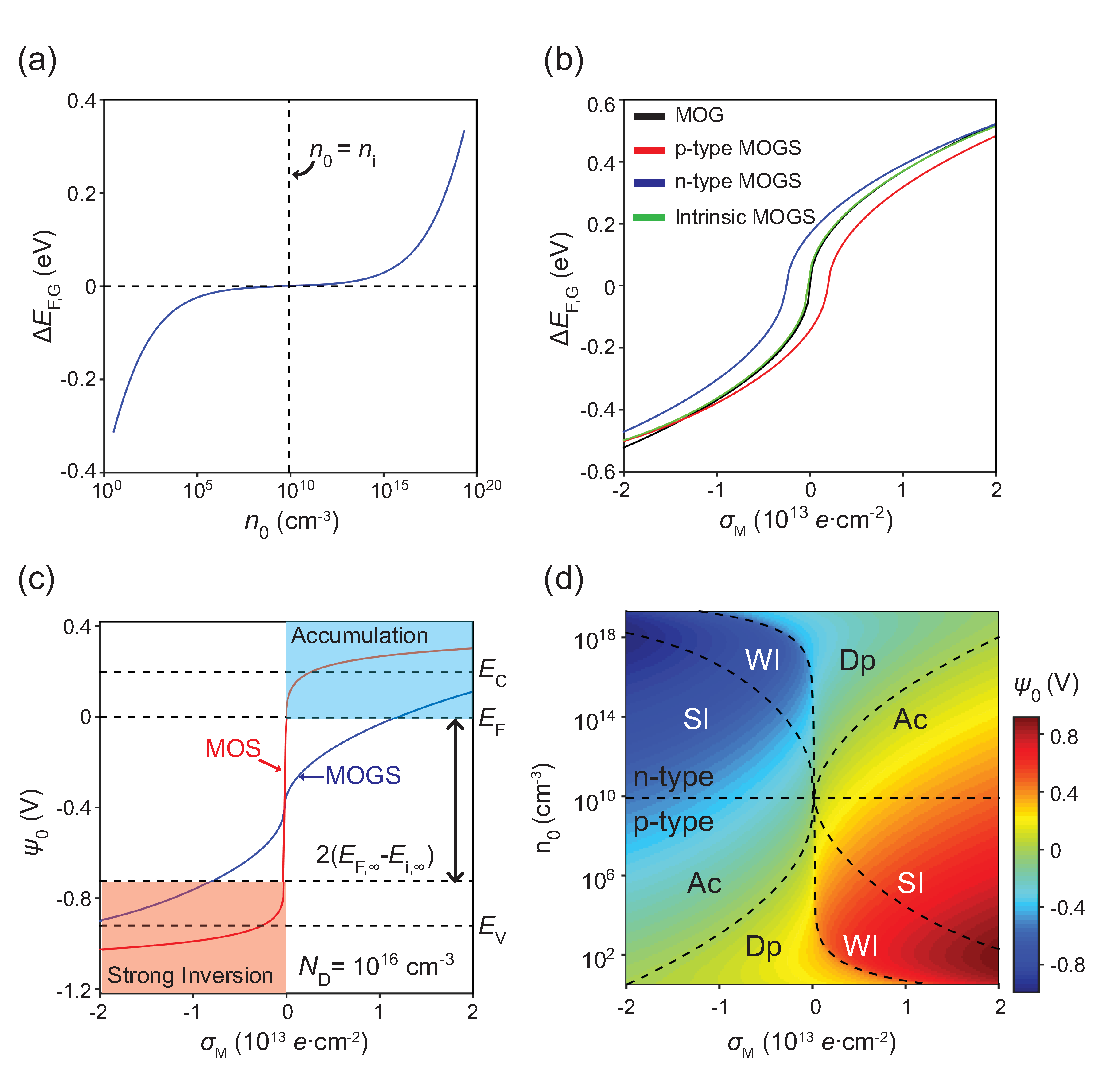
\includegraphics[width=0.95\linewidth]{img/FIG2.eps}
  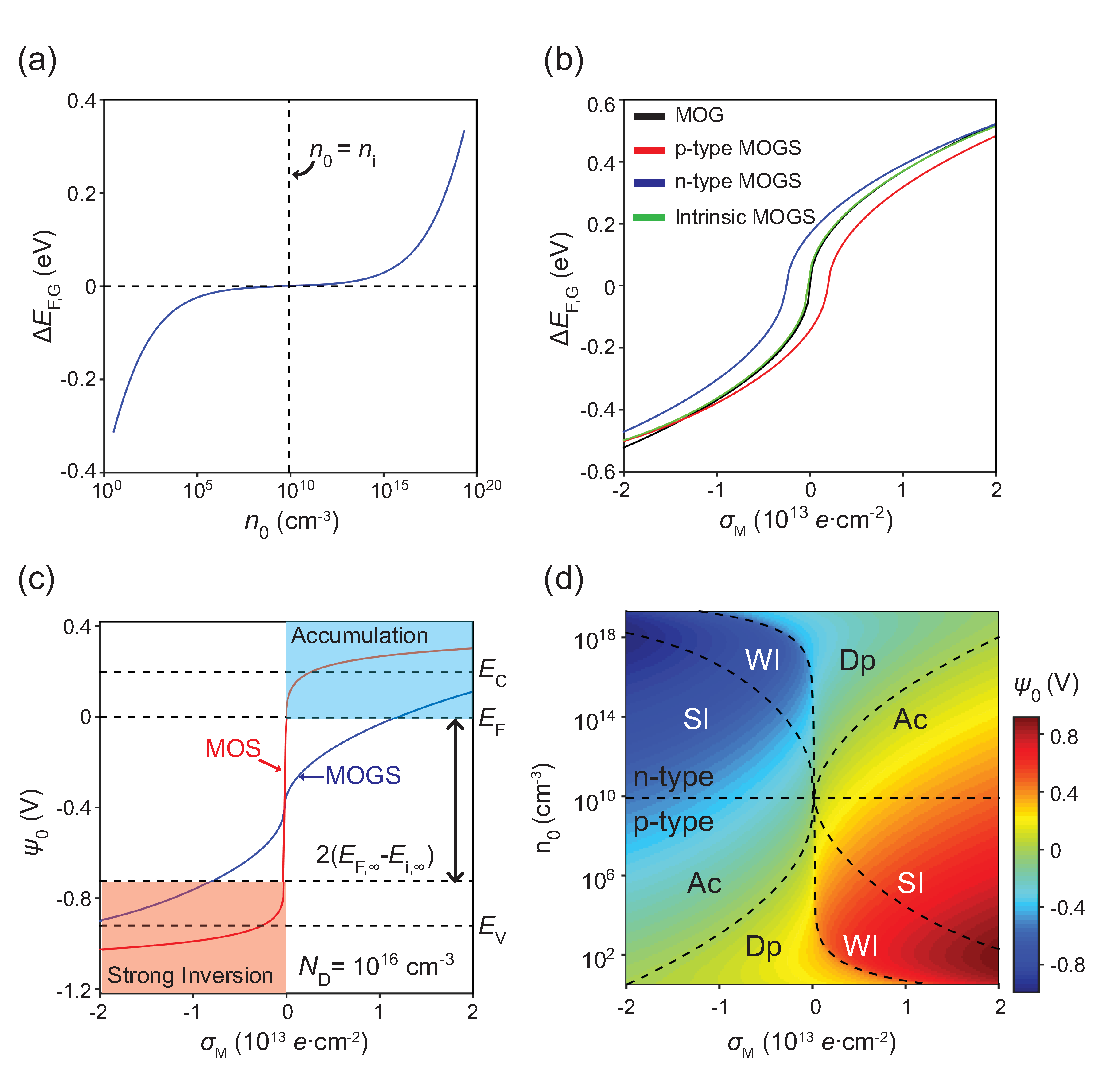
\includegraphics[width=0.95\linewidth]{img/FIG2.eps}
  % \caption{(a) Change of graphene's Fermi level as a function of $n_0$ in the Si layer. (b) Response of graphene's  Fermi level to $\sigma\subs{M}$, under different conditions (MOG QC; MOGS QCs consisted of intrinsic  Si and p-type / n-type Si with majority dopant concentration of 10$^{18}$ cm$^{−3}$, respectively). (c) $\psi_0$ as a function of $\sigma\subs{M}$ in MOS (red  line) and  MOGS QC(blue  line) consisted of n-type  Si with $N\subs{D}$=10$^{16}$  cm$^{−3}$.  The accumulation (light blue) and strong inversion (pink)  regimes are shown. (d) Contour map of  $\psi_0$ as a function of $\sigma\subs{M}$ and $n_0$, categorized into  accumulation (Ac), depletion  (Dp),  weak inversion (WI)  and strong  inversion (SI) regimes according to interface charge densities.}
  \caption{(a) The calculated Fermi level change of graphene, $\Delta E_{\mathrm {F,G}}$, as a function of $n_0$ in Si when 
  considering free contact between the graphene and Si layers.
  (b) The calculated $\Delta E_{\mathrm {F,G}}$ as a function of $\sigma\subs{M}$ in a MOG 
  capacitor and a MOGS QC. The doping level of majority carrier in p-type/n-type Si is 10$\sups{18}$ cm$\sups{-3}$.
  (c) The calculated $\psi_0$ as a function of $\sigma\subs{M}$ in n-type ($N\subs{D}=10^{16}$ cm$\sups{-3}$) MOS and MOGS capacitors. The accumulation (light blue) and strong inversion (pink) regimes are also shown for comparison.
  (d) The calculated contour map of $\psi_0$ as a function of $\sigma\subs{M}$ and $n_0$. The accumulation (Ac), depletion (Dp), weak inversion (WI), and strong inversion (SI) regimes are defined accordingly.
  }
  \label{fig:fermi-level-change}
\end{figure}

Next, we apply a nonzero $\sigma\subs{M}$ to the metal terminal, corresponding to a $V\subs{M}$ described by eq \ref{eqn:V_M}.
A proper range of $\sigma\subs{M}$ up to $\pm$2$\times$10$^{13}$ $e\cdot$cm$^{-2}$, which can be reached by using a high-k dielectric oxide layer \cite{Das2008Monitoring}.
$\sigma\subs{M}$ and $\sigma\subs{S}$ are subsequently altered as a result of the field effect.
The $\Delta E_{\mathrm {F,G}}$ - $\sigma\subs{M}$ curves at different silicon doping levels are shown in Figure \ref{fig:fermi-level-change}b.
By solving eq \ref{eqn:phi-gr} with $\sigma\subs{G}$ + $\sigma\subs{M}$ = 0, the curve associated with a MOG QC is also shown for comparison.
As well-stated in literature \cite{Neto2009Electron}, due to a small density of states (DOS) near the CNP of graphene, $\Delta E_{\mathrm {F,G}}$ changes rapidly as $\sigma\subs{M}\to0$ in the MOG QC.
In the range of $\sigma\subs{M}$ considered, one can tune the Fermi level of graphene up to $\pm$0.5 eV.
On the other hand, regarding the MOGS QCs in which graphene is in contact with a silicon layer, when an intrinsic Si is used, we do not find a notable difference until a relatively high $|\sigma\subs{M}|$ is applied. 
Nevertheless, when the Si layer is heavily doped (with a majority dopant concentration of 10$^{18}$ cm$^{-3}$), an considerable deviation from the $\Delta E_{\mathrm {F,G}}$ - $\sigma\subs{M}$ curve of MOG is observed.
It suggests that $\sigma\subs{G}$+$\sigma\subs{M}$ (which is equal to -$\sigma\subs{S}$ numerically) becomes nonzero, or in other words, the induced charges in graphene partially ``leak'' to the adjacent semiconductor layer.
We therefore suggest that the estimation of graphene's work function using $\phi\subs{G}|_{\sigma\subs{G}=-\sigma\subs{M}}$ in a MOGS QC, as has been widely used to estimate the work function of graphene in a MOGS QC (e.g. ref. \citenum{georgiou2013vertical}) appears to be incorrect.
Indeed, in a MOGS QC, graphene behaves like a 2DEG and is not capable of completely screening the electric displacement field applied.

In order to further understand the penetration of the field effect through graphene, Figure \ref{fig:fermi-level-change}c compares the evolutions of calculated $\psi_0$ with $\sigma\subs{M}$ in a standard metal-oxide-semiconductor (MOS) capacitor and a MOGS QC ($N\subs{D}$ = 10$\sups{16}$ cm$\sups{-2}$), as a function of $\sigma\subs{M}$.
In a standard MOS capacitor, the field effect allows to modulate the space charge concentration in the semiconductor layer significantly by applying a relatively small $\sigma\subs{M}$, such that $\psi_{0}$ changes rapidly and moves beyond the conduction and valence band energy levels ($E\subs{C}$ and $E\subs{V}$).
On the other hand, in a MOGS QC, the modulation of $\psi_0$ is observed to be less sensitive to $\sigma\subs{M}$, suggesting that the field effect only partially penetrates through graphene.
Nevertheless, one can still tune $\psi_0$ from the strong inversion regime (pink, corresponding to $p(x = 0) > N\subs{D}$) to the accumulation regime (light blue, corresponding to $n(x = 0) > N\subs{D}$), but not to the band edges. 
Clearly, unlike the standard MOS capacitors, we predict that the MOGS QC devices inherently do not facilitate fast switching by the field effect.

Another important observation in Figure \ref{fig:fermi-level-change}b is that $\sigma\subs{G}$ also depends on the doping level of the adjacent Si layer.
In order to further discuss this effect, Figure \ref{fig:fermi-level-change}d presents the contour map of $\psi_0$   as functions of $\sigma\subs{M}$ and $n_0$. 
We also include three curves associated with: (i) $\psi_0=0$, (ii) $\psi_0= -( E_{\mathrm F,\infty} - E_{\mathrm i,\infty})/e$, and (iii) $\psi_0 = -2(E_{\mathrm F,\infty} - E_{\mathrm i,\infty})/e$, where $E_{\mathrm i,\infty}$ is the intrinsic energy level of semiconductor at the flat-band condition.
Note that the three curves intersect at ($n\subs{i}$, $\sigma\subs{M}^0$), in which $\sigma\subs{M}^0$ is given by
\begin{align}
    \sigma\subs{M}^0 = \mathrm{sign}(\phi\subs{G}^0-\phi\subs{S}^0)\frac{(\phi\subs{G}^0-\phi\subs{S}^0)^2 e^3}{\pi \hbar^2 v\subs{F}^2}
\end{align}
where $\phi\subs{S}^0$ is the work function of intrinsic semiconductor. 
Following the convention in semiconductor physics \cite{Sze2006Mosfets}, the three curves divide the contour map into four regimes as follows: (i) the accumulation (Ac), (ii) the depletion (Dp), (iii) the weak inversion (WI), and (iv) the strong inversion (SI). 
As shown, within the $\sigma\subs{M}$ range considered, the partially-penetrated field effect allows the induction of an inversion or accumulation layer at the SG interface, unless the semiconductor doping level is relatively high (with an majority carrier concentration $> 10^{18}$ cm$^{-3}$).
The wide tunability results from the following two facts: (i) $\sigma\subs{S}^0$ is very close to $\sigma\subs{G}^0$, and (ii) the bandgap is comparable to the tunable range of $E_{\mathrm {F,G}}$. 
Our findings explain why Si has been considered as a good semiconductor candidate in the MOGS QCs \cite{Yang2012Graphene, Regan2012ScreeningEngineered}.

%\todo[inline]{PARAGRAPHS FOR FIRST PRINCIPLE CALCULATIONS }

% $\sigma_{\rm G,Si}=\sigma ()$  Blue and red isosurfaces represent positive and negative charge. $\sigma_{Si}(10^{13}$ cm$^{-2})$) = \sim 0.98$.





Based on the above analysis, we propose and derive an expression for the index $\eta$ that quantifies the degree of transparency to an electric displacement field in a MOGS QC as follows:
\begin{align}
    \eta = -(\frac{\partial \sigma\subs{S}}{\partial \sigma\subs{M}})
    \label{eqn:def_eta}
\end{align}
\begin{figure}[htbp]
  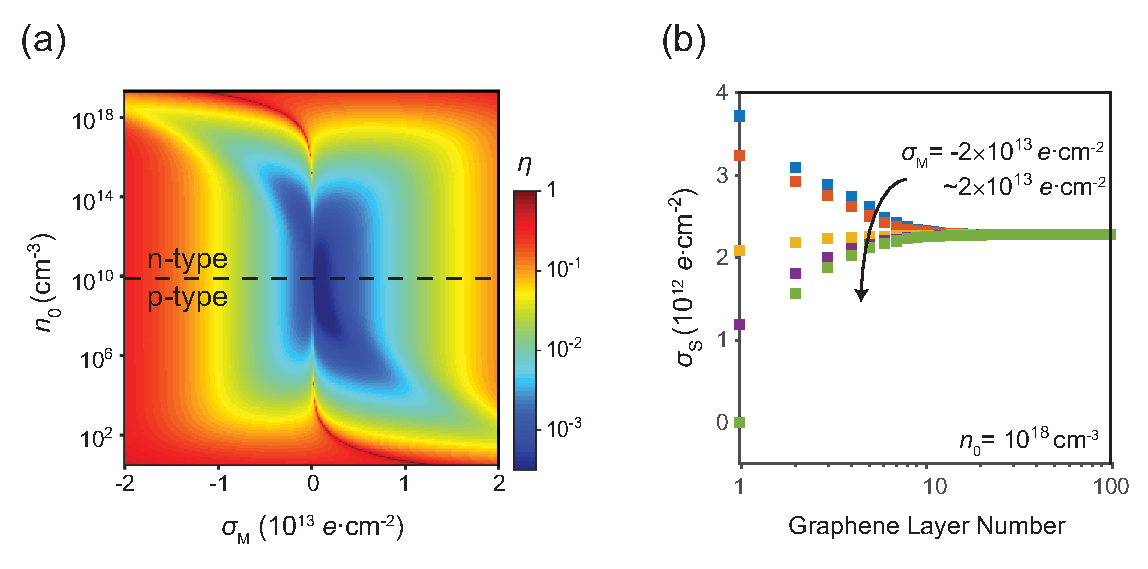
\includegraphics[width=0.9\linewidth]{img/FIG3.eps}
  \caption{(a) Calculated transparency of graphene 2DEG to electric displacement field in a MOGS QC, as functions of $\sigma\subs{M}$ and $n_0$. 
  \change{(b) Calculated $\sigma\subs{S}$ as a function of number of graphene layers in a MOGS QC ($n\subs{0}=10^{18}$ cm$\sups{-3}$). The arrow indicates the direction of increasing $\sigma\subs{M}$.}
  }
  \label{fig:transparency-MOGS}
\end{figure}
We can deduce that $-(\partial \sigma\subs{G} / \partial \sigma\subs{M})=1-\eta$, and by taking that (i) $(\partial \phi\subs{G}/\partial \psi\subs{S})=-1$ (see eq \ref{eqn:Shottky-Mott}), (ii) the quantum capacitance of graphene $C\subs{G}=\partial \sigma\subs{G} / \partial \phi\subs{G}$ and (iii) the capacitance of semiconductor $C\subs{S}  = -(\partial \sigma\subs{S}/ \partial \psi_0)$, the transparency index $\eta$ in eq \ref{eqn:def_eta} can be decomposed using the chain rule and follows
\begin{equation}
  \label{eqn:eta_expanded}
    \begin{aligned}
      \eta &= \left(\frac{\partial \sigma\subs{S}}{\partial \psi_0}\right) \left(\frac{\partial \sigma\subs{G}}{\partial \phi\subs{G}}\right)^{-1} \left(\frac{\partial \sigma\subs{G}}{\partial \sigma\subs{M}}\right)\\
          &= \frac{1}{1+C\subs{G}/C\subs{S}}= (1+\frac{2}{\hbar v\subs{F}} \sqrt{\frac{e^3 |\sigma\subs{G}|}{\pi}}\frac{\mathscr{E}_0}{\rho_0})^{-1}
    \end{aligned}
\end{equation}
where $\rho_0$ is the charge density at the SG interface.
\change{
We also consider the effect of interface states on the transparency of graphene (see Supporting Information), 
which suggests that the existence of an interfacial layer reduces the transparency.
In practice, although the interface states are difficult to be removed completely, their influence can be minimized by creating a clean semiconductor surface with minimal interfacial contamination \cite{withers2015light}.
Thereafter we still use the expression of eq \ref{eqn:eta_expanded} to simplify the following analysis. 
}


Accordingly, the contour map of $\eta$ as a function of $\sigma\subs{M}$ and $n_0$ is shown in Figure \ref{fig:transparency-MOGS}a.
Eq \ref{eqn:eta_expanded} suggests that the transparency of graphene 2DEG to an electric displacement field is determined by the combined effects of the graphene quantum capacitance and the semiconductor capacitance.
As a result, the limit of perfect transparency, $\eta \to 1$, occurs when $C\subs{G} \to 0$, corresponding to the CNP of graphene, along the curve of $\psi_0=0$ in Figure \ref{fig:fermi-level-change}d. 
However, we observe that this transparency disappears by slightly changing $\sigma\subs{M}$, due to the rapid increase of  $\phi\subs{G}$ with $\sigma\subs{G}$ near the CNP of graphene \cite{Neto2009Electron}.
In practice, considering the residual charges induced by the electron-hole puddles near the CNP of graphene \cite{Sarma2011Electronic}, we predict that the limit of $\eta \to 1$ may not be observable experimentally.
On the other hand, a general trend exhibited in Figure \ref{fig:transparency-MOGS}a is that one can gain a higher degree of transparency for the graphene 2DEG by: (i) increasing the doping level in the Si layer, and (ii) applying a higher $|\sigma\subs{M}|$, resulting a considerable increase of $C\subs{S}$.
\change{
  We can further conclude from eq \ref{eqn:eta_expanded} that when the graphene layer number increases, the field-effect transparency would be attenuated. 
  Intuitively speaking, the total DOS of multilayer graphene increases with the layer number and results in a larger $C\subs{G}$ value. In the case of graphite with infinite layers of graphene, the electric displacement field is completed screened and $\sigma\subs{S}$ becomes independent of $\sigma\subs{M}$.
  Here, instead of deriving the total DOS of multilayer graphene by the tight-bonding model \cite{Nilsson2008} or \textit{ab initio} calculations, 
  we propose a simplified model, which assumes that the interlayer coupling is neglegible and each layer behaves as monolayer graphene (see details in Supporting Information).
  The $\sigma\subs{S}$ calculated under different $\sigma\subs{M}$ as a function of graphene layer number are shown in Figure \ref{fig:transparency-MOGS}b.
  We observe that $\sigma\subs{S}$ becomes independent of $\sigma\subs{M}$ when more than 10 layers of graphene are used in the MOGS QC, and consequently, the transparency decays to nearly zero with graphene layer number (Supporting Information Figure S5).
  This is in agreement with the non-linear nature of the screening in multilayer graphene \cite{Santos2013Graphene}, which shows a high polarization charge at a few graphene layers adjacent to an external electric displacement field, while the charge in graphene decays exponentially in deeper layers.  
}              
%First-principles paragraph 

The above analysis based on Poisson-Boltzmann equation methods is still valid at different levels of theory as calculated using first-principles methods within density functional theory (DFT) including 
van der Waals interactions (see {\it Methods} for details). 
\begin{figure}[htbp]
  % 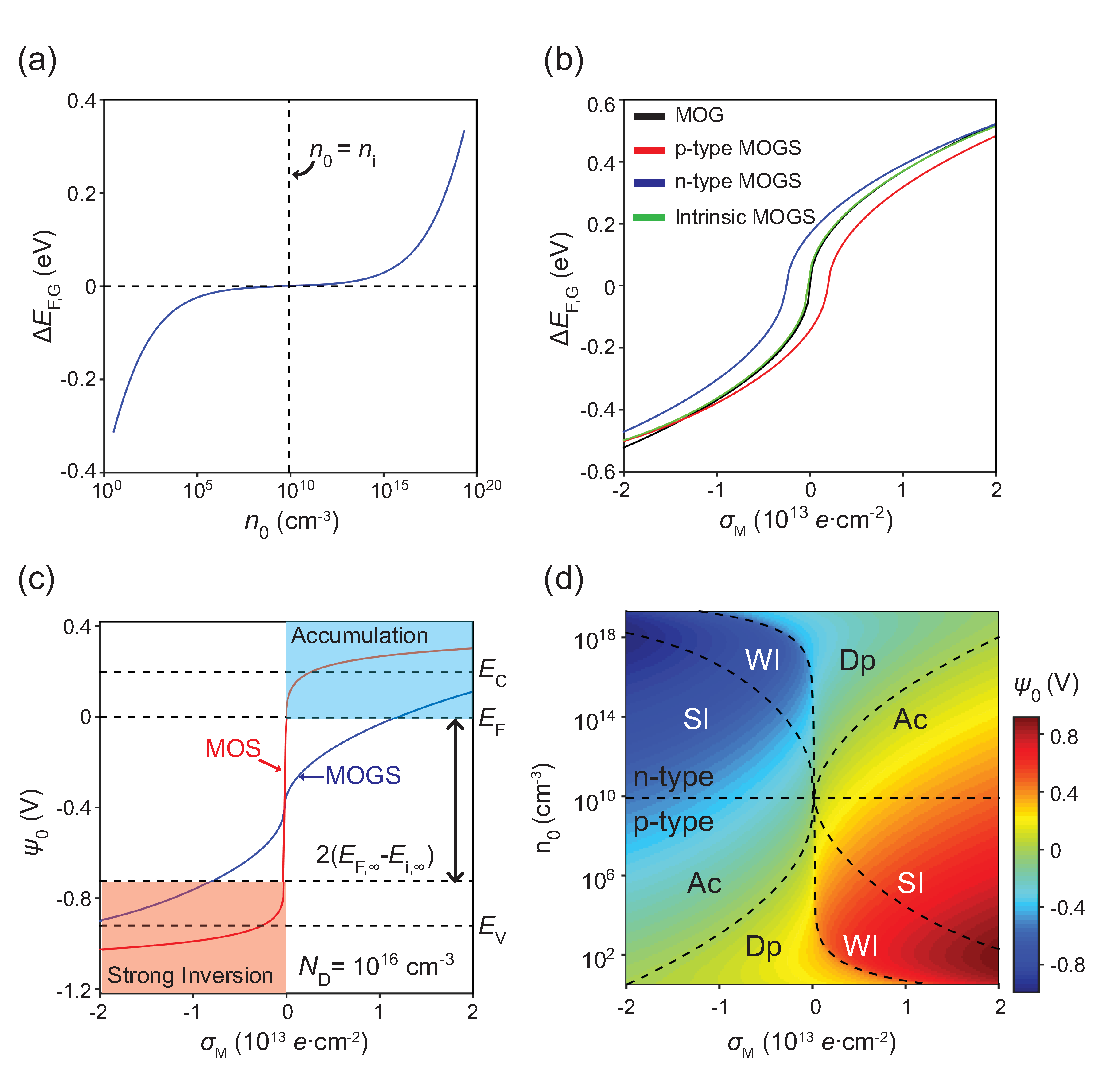
\includegraphics[width=0.95\linewidth]{img/FIG2.eps}
  \includegraphics[width=0.95\linewidth]{img/FIG4.eps}
  \caption{Induced charge densities at (a) graphene, $\sigma\subs{G}$, and (b) Si(111), $\sigma\subs{S}$, as a function of $\sigma\subs{M}$ in different systems: intrinsic (blue), p-type (green)  and n-type (red) Si, respectively.
  The average carrier numbers per unit area in the whole Si slab are $1.10\times10^{13}$ cm$\sups{-2}$ for p-type Si and $-1.10\times10^{13}$ cm$\sups{-2}$ for n-type Si. 
  (c) Total average charge density cross 
  section $\Delta \rho\subs{tot}$
  as a function of the coordinate $x$ perpendicular to the graphene/Si(111) interface. 
  The positions of graphene and Si(111) are marked with the underneath faint structure. 
  The color gradient shows the evolution of $\sigma\subs{M}$ as displayed on the right side. Molecular visualizations of the induced charge density in graphene and intrinsic Si layers
  (cutoff at $\pm 0.0021$ $e\cdot$Bohr$^{-3}$) when (d) $\sigma\subs{M}=-0.98\times10^{13}$ cm$\sups{-2}$ and (e) $\sigma\subs{M}=0.98\times10^{13}$ cm$\sups{-2}$. 
  Blue and red isosurfaces represent positive and negative charges, respectively.
  %\protect \todo[inline]{Is the description for doping density right?} 
  }
  \label{fig:first principle}
\end{figure}
Figure \ref{fig:first principle} shows the calculated electronic response on a graphene/Si(111) interface considering the effect of $\sigma\subs{M}$. 
%\todo[inline]{Should we describe the layers of Si used here?}
% We find that there is a neutrally systematic tuning of the induced charge into 
% system as a function of $\sigma\subs{M}$ irrespective of the doping level considered (Fig. \ref{fig:first principle}a and b). 
We find that, irrespective of the doping levels considered, both $\sigma\subs{G}$ and $\sigma\subs{S}$ monotonically decrease as $\sigma\subs{M}$ increases (Fig. \ref{fig:first principle}a and b).
Similar to Figure \ref{fig:fermi-level-change}b, the amount of induced charges in both graphene and Si layers as a result of $\sigma\subs{M}$ can be deviated by different doping levels of Si.
These results indicate that the graphene 2DEG is also transparent to the electric displacement field from the first-principles calculations.
We also observe that both $\sigma\subs{G}$ and $\sigma\subs{S}$ show a nearly linear relation with $\sigma\subs{M}$ when very high $\sigma\subs{M}$ (up to $\pm20\times10^{13}$ $e\cdot$cm$^{-2}$) is applied (Supporting Information Figure S1), which allows us to extract the $\eta$ by performing a linear-fitting to the $\sigma\subs{S}-\sigma\subs{M}$ curves using 
the formula $\sigma\subs{S}=-\eta \sigma\subs{M} + b$, where $b$ is a constant.
Interestingly, regardless of the Si doping level, all three systems shown a $\eta$ near 0.70.
This observations can be explained by the concept of transparency in eq \ref{eqn:eta_expanded}. 
The few-layer Si behaves more like a 2D than bulk material, of which the quantum 
capacitance $C\subs{S}$ remains almost constant when charges are filled into its 
valence band (VB) or conduction band (CB) \cite{Davies1997Physics}.
Conversely, when the doping level of graphene is extremely high, its quantum capacitance $C\subs{G}$ will be less dependent of the charge density after the van Hove singularity is reached \cite{Sarma2011Electronic}. 
According to eq \ref{eqn:eta_expanded}, $\eta=(1+C\subs{G}/C\subs{S})^{-1}$, due to that $C\subs{G}$ and $C\subs{S}$ are nearly constant, the $\eta$ value becomes independent of either $\sigma\subs{M}$ or Si doping level.
Moreover since $C\subs{S}$ is essentially larger than $C\subs{G}$ in this case as a result of higher DOS of Si in the VB and CB, it is plausible to have a $\eta$ larger than 0.5.
We also study the charge distribution over the SG interface as a function of $\sigma\subs{M}$, which exhibits an intriguing profile as shown in Figure \ref{fig:first principle}c. 
At both positive and negative $\sigma_{\rm M}$ regimes, the induced charge density cross section of the system $\Delta \rho\subs{tot}$ shows a higher accumulation at the graphene surface than in the Si slab, due to different electronic behaviors of both materials, namely, semimetallic versus semiconducting. 
A nonlinear pattern is clearly observed throughout the semiconductor slab, 
as a result the carriers in the Si layer are accumulated in the vicinity of the SG interface.
Molecular visualizations of this effect are shown in Figure \ref{fig:first principle}d and \ref{fig:first principle}e for a graphene layer and an intrinsic Si slab.
It is found that that most of the orbitals that contribute to the polarization of charge are the $2p\subs{z}$ in graphene and 
$3p\subs{z}$ in Si, dependent on the polarity of $\sigma\subs{M}$ applied. 
According to the results above, we find a good consistency between the macroscopic model and first-principles calculations, which allows us to perform a multiscale analysis for the transparency of graphene 2DEG to an electric displacement field. 
        

The interesting behavior at the interface 
has drawn our attention to the possibility of replacing graphene in a MOGS QC structure with other 2D materials. 
Indeed, as addressed earlier, the ultra-thinness of these materials suggests good potential for 2DEGs.
Under the assumption that a 2D material-semiconductor interface satisfies the Schottky-Mott rule, it is suggested that the relation of  $\eta=(1+C\subs{Q}/C\subs{S})^{-1}$ still holds (here $C\subs{Q}$ substitutes $C\subs{G}$ for quantum capacitance in general 2D materials).  
Since the quantum capacitance can be expressed as $C\subs{Q}=g(E) e^2$ \cite{john2004quantum}, 
where $g(E)$ is the DOS at a certain energy level $E$, 
we have calculated the DOS as a function of $E$ for a variety of 
2D materials\cite{Xu2011Measurements, Jimenez2012drift, Nawaz2016quantum} using the 
density functional theory (see Supporting Information Figure S2). We also take 
into account 
a fractional component of the exact exchange from the Hartree-Fock (HF) theory
hybridized with the DFT exchange-correlation functional at the level of the 
HSE06 hybrid functional\cite{HSE06} (see {\it Methods}). Therefore any limitation of 
the exchange and correlation functional utilized in the chemical description of the energy levels can be improved. 
\begin{figure}[htbp]
  \centering
  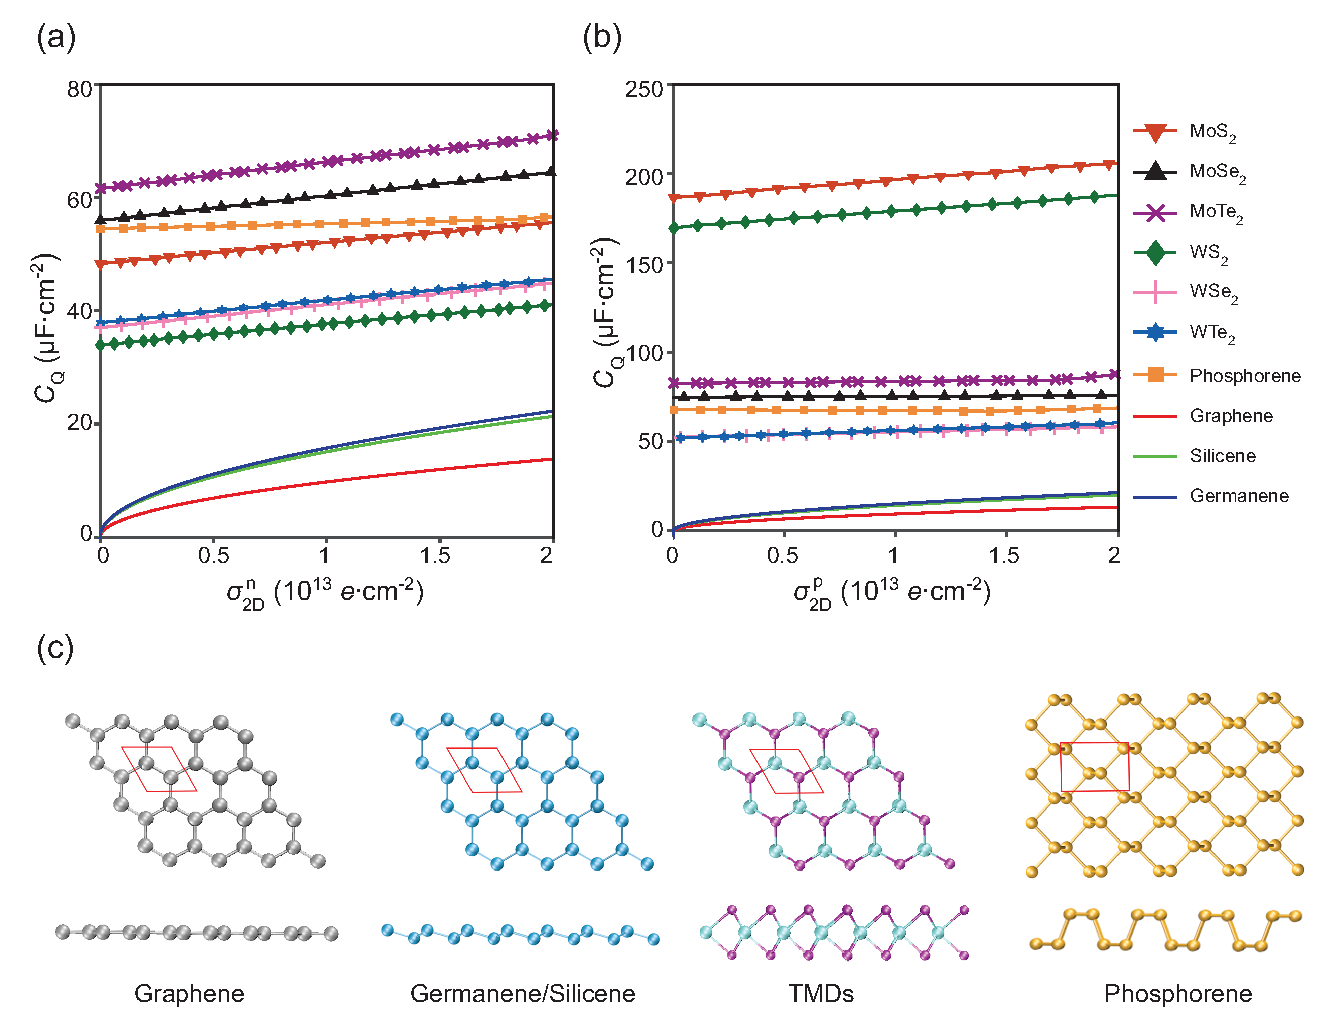
\includegraphics[width=0.95\textwidth]{img/FIG5.eps}
  \caption{
  \change{
  Calculated quantum capacitances ($C\subs{Q}$) for the 2D 
  materials considered, TMDs (MX$\subs{2}$, M = Mo, W; X = S, Se, Te), phosphorene, silicene, germanene and graphene,  
  as a function of the (a) electron density $\sigma\subs{2D}\sups{n}$ and (b) hole density $\sigma\subs{2D}\sups{p}$. 
  (c) Geometries used to calculated 
  the QC using HSE06 hybrid functional for graphene, silicene/germanene, TMDs and phosphorene. 
  The unit cell used in the simulations is highlighted in the panels. 
  } 
 }
  \label{fig:CQ-2D}
\end{figure}
% The relation between DOS and quantum capacitance 
% enables us to compare the transparency of a large variety of 2D electronic materials 
% in metal-oxide-2D material-semiconductor heterostructure through their DOS profiles.
The following 2D materials are considered:  transition metal dichalcogenide (TMD) 
monolayers (MX$\subs{2}$, M = Mo, W; X = S, Se, Te), silicene (2D allotrope of Si), germanene (2D allotrope of Ge)
\change{
  and phosphorene (monolayer black phosphorus, 2D allotrope of P)
}.
The charge density in a 2D material is calculated by integrating the DOS from its intrinsic Fermi level, i.e., $\sigma\subs{2D}=\int_{E\subs{F}}^{E}  g(E')e dE'$.
The calculated quantum capacitances for the 2D materials considered as a function of the electron or hole density are shown in Figure \ref{fig:CQ-2D}a and \ref{fig:CQ-2D}c, respectively. 

The quantum capacitance of a monolayer 2D semiconductor (\change{TMDs and phosphorene}) behaves like a step function and only increases gradually with $\sigma\subs{2D}$, close to that for an ideal 2D semiconductor \cite{Davies1997Physics}. 
On the other hand, the quantum capacitance of a 2D semimetal, including graphene, silicene, and germanene, exhibits a quadratic relation with respect to $\sigma\subs{2D}$, because they share the same feature of linear $E-k$ dispersion. 
More importantly, the quantum capacitance for the 2D semimetals are always less than those for the 2D semiconductors under the same charge density. In other words, although there is no states in the band gap, the DOS above the band edge in a 2D semiconductor is significantly higher compared to that in a semimetal, reflecting the fact that the effect mass of carriers in the 2D semiconductors is much higher than that in the 2D semimetals \cite{Davies1997Physics}. 
This concept also explains why the $C\subs{Q}$ for silicene and germanene are similar but higher than that in graphene. Indeed, recent reports have suggested that the Fermi velocities, $v\subs{F}$, in silicene and germanene are only about 60\% of that in graphene \cite{yan2013electron,bechstedt2012infrared}. 
combining with eq \ref{eqn:eta_expanded}, the observations have led to the conclusion that graphene exhibits the highest transparency to an electric displacement field among all the 2D materials considered here.
The theoretical framework also allows us to rank the 2D materials according their transparency. For example, when the majority carrier is electron, the following rank is predicted: 
\change{graphene > silicene > germanene > WS$\subs{2}$ > WTe$\subs{2}$ > WSe$\subs{2}$ > MoS$\subs{2}$ > phosphorene > MoSe$\subs{2}$ > MoTe$\subs{2}$.
}
\change{
The above analysis for field-effect transparency through multilayer graphene can also be applied to other 2D materials. 
Indeed, the total DOS of a multilayer 2D material increases with layer number, leading to a higher $C\subs{Q}$ and consequently lower field transparency.
}

Finally, we discuss the effect of the bias $V\subs{b}$ between the semiconductor and graphene terminals.
Eqs \ref{eqn:sigma_S_exact} and \ref{eqn:Shottky-Mott}  have suggested that a nonzero $V\subs{b}$ changes $\psi_0$ and $\sigma\subs{S}$, and in order to satisfy the electroneutrality of the system imposed by eq \ref{eqn:charge-balance}, an adjustment of the graphene's work function $\phi\subs{G}$ occurs, unlike that in a semiconductor-metal (SM) interface. 
Specifically, Figure \ref{fig:chara-bias}a illustrates the main differences between SM and SG interfaces. 
In a semiconductor-metal (SM) junction, the Schottky barrier height $\phi\subs{b}$ remains constant ($\phi\subs{b}^0$) with $V\subs{b}$, because the work function of metal is independent of its charge density. 
As a result, the surface potential in the semiconductor layer increases linearly with $V\subs{b}$ \cite{Sze2006Mosfets}.
On the contrary, in an semiconductor-graphene (SG) junction, under a reverse bias with $V\subs{b}$ > 0, compare to that with zero bias, one can expect a more negative $\mathscr{E}_0$, followed by an increase of $\sigma\subs{S}$.
It is the other way around for $V\subs{b}$ < 0. As a result, one can expect that $\sigma\subs{G}$, as well as the resulting $\psi_0$ and $\phi\subs{b}$, exhibit a nonlinear dependence on $V\subs{b}$. 
\begin{figure}[htbp]
  \centering
  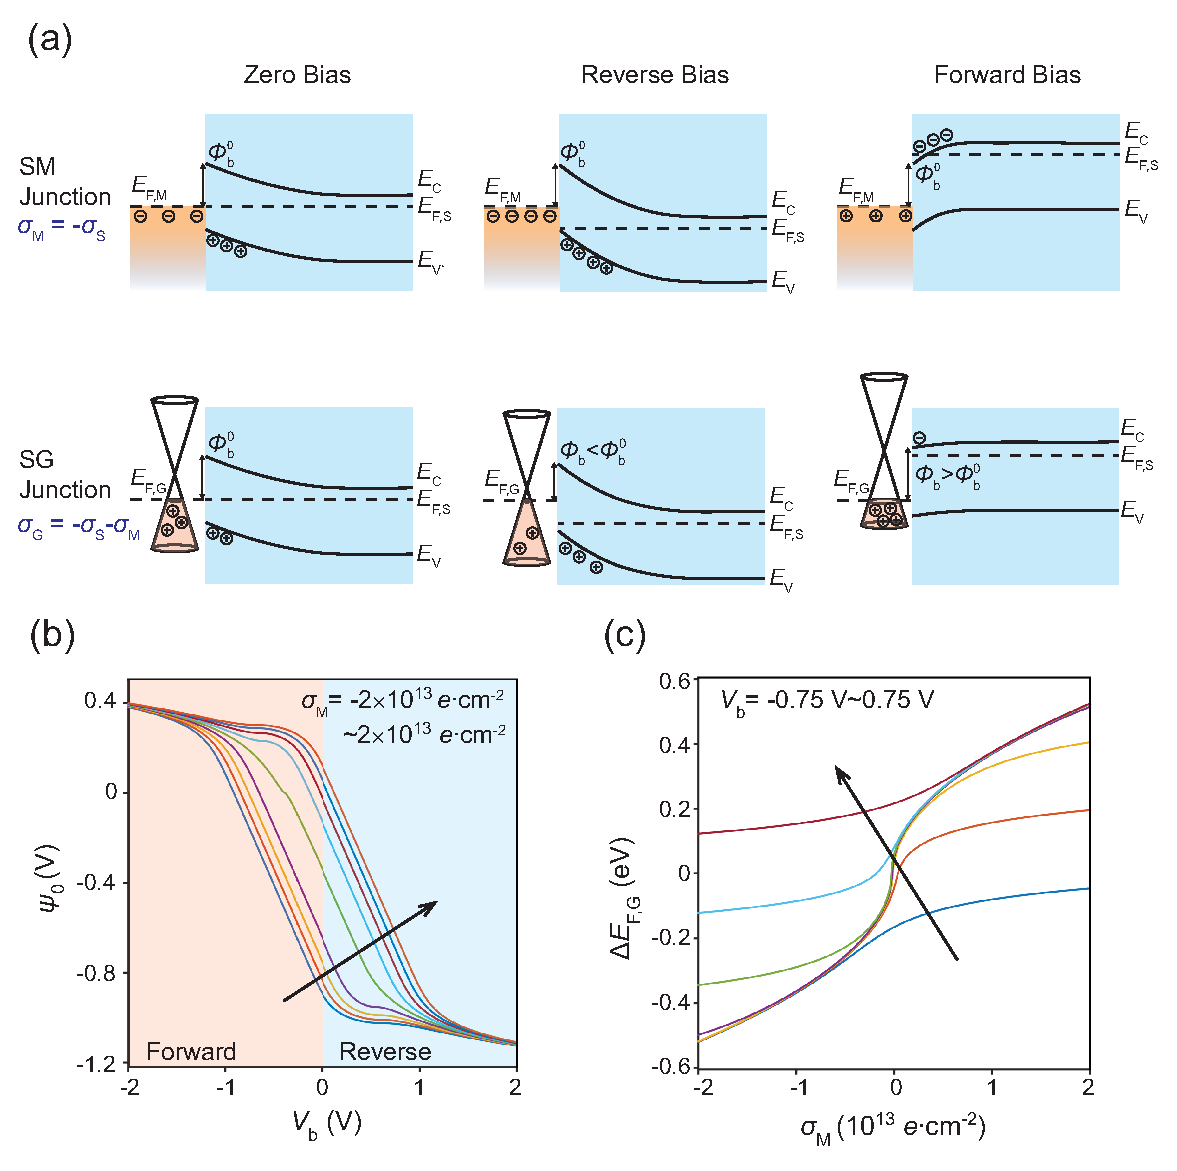
\includegraphics[width=0.95\linewidth]{img/FIG6.eps} %for preprint
  % \caption{Characterizations of a MOGS QC when an bias is applied. (a) Illustration of the difference between a metal-semiconductor (M-S) and a graphene-semiconductor (G-S) junction. (b) $\psi_0$ as a function of $V\subs{b}$, in case of  varied gate charge densities $\sigma\subs{M}$. The MOGS QC consists of a Si layer with $N\subs{D}$=10$^{16}$ cm$^{-3}$. $\sigma\subs{M}$  varies from -2$\times$10$^{13}$  $e\cdot$cm$^{-2}$ to 2$\times$10$^{13}$  $e\cdot$cm$^{-2}$ , with  a step  of 5$\times$10$^{12}$  $e\cdot$cm$^{-2}$.  The  arrow indicates  the  direction  of increasing $\sigma\subs{M}$ .  (c)  $\Delta E_{\mathrm {F,G}}$  in the same MOGS QC discussed in (b) as a function of  $\sigma\subs{M}$ when different values of $V\subs{b}$ are applied. $V\subs{b}$  ranges  from -0.75 V to  0.75 V, stepped  by 0.25 V. The arrow indicates  the direction  of increasing $V\subs{b}$.}
  \caption{
  The effect of $V\subs{b}$ in a MOGS QC. (a) Schematic illustration of the difference between a semiconductor-metal (SM) and a semiconductor-graphene (SG) junction.
  (b) Calculated $\psi_0$ as a function of $V\subs{b}$, under different $\sigma\subs{M}$ values. The  arrow indicates  the  direction  of increasing $\sigma\subs{M}$.
  (c) Calculated $\Delta E_{\mathrm{F,G}}$ as a function of $\sigma\subs{M}$ under different $V\subs{b}$ values. The  arrow indicates  the  direction  of increasing $V\subs{b}$.
  A n-type Si with $N\subs{D}=10^{16}$ cm$^{-3}$ is considered for (b) and (c).
  }
  \label{fig:chara-bias}
\end{figure}

Taking a MOGS QC using an n-type silicon ($N\subs{D} = 10^{16}$ cm$^{-3}$) as an example, the calculated $\psi_0$ as a function of $V\subs{b}$ under various $\sigma\subs{M}$ values applied is shown in Figure \ref{fig:chara-bias}b.
Compared to the case of $V\subs{b} = 0$, in which a relatively wide range of $\psi_0$ can be tuned by $\sigma\subs{M}$, it is found that, by increasing $|V\subs{b}|$, in both forward and reverse bias regimes, $\psi_0$ becomes less tunable by $\sigma\subs{M}$, or in other words, $\sigma\subs{M}$ is losing control over the graphene's Fermi level $E_{\mathrm {F,G}}$, when a higher $|V\subs{b}|$ is applied. 
We rationalize this observation by evaluating $E_{\mathrm {F,G}}$ with respect to $\sigma\subs{M}$ under constant $V\subs{b}$, or namely, $(\partial E_{\mathrm {F,G}}/\partial \sigma\subs{M})_{V\subs{b}}$.
Using $(\partial \phi\subs{G}/\partial \psi_0)_{V\subs{b}}=-1$ (see eq \ref{eqn:Shottky-Mott}) and eq \ref{eqn:eta_expanded}, it follows:
\begin{equation}
  \label{eqn: tunability_gate}
  \begin{aligned}
      \left(\frac{\partial E_{\mathrm {F,G}}}{\partial \sigma\subs{M}}\right)_{V\subs{b}} &= -\left(\frac{\partial \phi\subs{G}}{\partial \sigma\subs{M}}\right)_{V\subs{b}} = \left(\frac{\partial \psi_0}{\partial \sigma\subs{S}}\right)_{V\subs{b}} \left(\frac{\partial \sigma\subs{S}}{\partial \sigma\subs{M}}\right)_{V\subs{b}}\\
      &= \frac{\eta}{C\subs{S}} = \frac{1}{C\subs{G}+C\subs{S}}= (\frac{2}{\hbar v\subs{F}} \sqrt{\frac{e^3 |\sigma\subs{G}|}{\pi}} + \frac{\rho_0}{\mathscr{E}_0})^{-1}
  \end{aligned}
\end{equation}
Considering only a slight degree of band bending at $|V\subs{b}|$=0, as shown in Figure \ref{fig:chara-bias}a, when a high forward or reverse $|V\subs{b}|$ is applied, an inversion or accumulation layer is formed at the SG interface due to a high degree of band bending, which essentially increases the capacitance of semiconductor $C\subs{S}$. 
In order to balance the induced $\sigma\subs{S}$, $\sigma\subs{G}$ also increases, thereby yielding a higher $C\subs{G}$. 
As suggested by eq \ref{eqn: tunability_gate}, a simultaneous rise of $C\subs{S}$ and $C\subs{G}$ under a high $|V\subs{b}|$ results in a significant decrease of $(\partial E_{\mathrm {F,G}}/\partial \sigma\subs{M})_{V\subs{b}}$, or the tunability of $E_{\mathrm {F,G}}$ with respect to $\sigma\subs{M}$, as shown in Figure \ref{fig:chara-bias}c. 
Representative band diagrams of a MOGS QC are shown in Supporting Information Figure S3.
This finding is consistent with the experimental observations that the on/off current ratio is lowered by applying a higher drain bias in a graphene-based vertical transistors \cite{Yang2012Graphene, yu2013vertically, georgiou2013vertical, Shih2015PartiallyScreened, Schwierz2010Graphene}.
That is to say, we suggest that the gate-tunable characteristics in a MOGS QC are only observable in a certain $|V\subs{b}|$ range.
To our knowledge, this effect has not been well discussed in literature.
 
In conclusion, we have presented the first multiscale approach to understand the penetration of the field effect through a monolayer 2D material in a metal-oxide-2D material-semiconductor quantum capacitor. 
By using graphene as the model system, first we develop a macroscopic model to describe the charge distribution in graphene and the semiconductor layers by applying a $\sigma\subs{M}$ on the metal electrode. 
Depending on the degree of $\sigma\subs{M}$, the space charge density in the semiconductor layer is modulated in a nonlinear manner, forming an accumulation or inversion layer at the semiconductor/graphene interface, which suggests that graphene is partially ``transparent'' to an electric displacement field. These results are corroborated by {\it ab initio} calculations at the level of density functional theory including van der Waals 
interactions. 

We therefore define and formulate the degree of transparency of a monolayer 
2D material to an electric displacement field, $\eta$, and show that $\eta$ is determined 
by the combined effect of graphene quantum capacitance and the semiconductor capacitance.
By calculating the quantum capacitance for a variety of 2D materials using hybrid functionals, we predict 
the ranking for a variety of 2D compounds according to their transparency to an 
electric displacement field 
as follows: 
\change{
graphene > silicene > germanene > WS$\subs{2}$ > WTe$\subs{2}$ > WSe$\subs{2}$ > MoS$\subs{2}$ > phosphorene > MoSe$\subs{2}$ > MoTe$\subs{2}$,
} when the majority carrier is electron. 
Finally, the effect of the voltage applied between the semiconductor and graphene terminals $V\subs{b}$ is discussed. 
Because a significant increase of the semiconductor capacitance with $|V\subs{b}|$ in either 
reverse or forward bias regime, we find that the 
gate-tunable characteristics in a MOGS QC are only effective in a certain $|V\subs{b}|$ range, 
which is often ignored in previous reports. 
We believe that the development of 2D materials-based quantum capacitors and 
vdW heterostructures will be greatly facilitated by the fundamental 
principles and theoretical analysis presented here.


\section{Methods}
The first-principles simulations reported here are based on density functional theory calculations 
using the  {\sc SIESTA} method\cite{soler02}  and the {\sc VASP} code\cite{kresse93,kresse96}. 
The generalized gradient approximation\cite{pbe-functional} along with 
non-local van der Waals density functional for the exchange-correlation term\cite{Dion-vdW}
have been used. A double-$\zeta$ polarized basis set in {\sc SIESTA}, and a well-converged plane-wave 
cutoff of 400 eV in {\sc VASP} were utilized in the calculations. Projected augmented wave 
method (PAW)\cite{Blochl94,kresse99} for the latter, 
and norm-conserving Troullier-Martins pseudopotentials\cite{troullier91} for the former, 
have been used in the description of the bonding environment at the different systems. 
Atomic coordinates were allowed to relax until the forces on the ions 
were less than 0.04 eV/\AA~under the conjugate gradient algorithm. 
Further relaxations (0.01 eV/\AA) do not change appreciably the energetics and geometries. 
To avoid any interactions between supercells in the non-periodic direction, a 15 \AA~vacuum space was 
used in all calculations. In addition to this, a cutoff energy of 150 Ry was used to resolve 
the real-space grid used to calculate the Hartree and exchange-correlation contribution to the total energy. 
A basis set of numerical atomic orbitals obtained 
from the solution of the atomic pseudopotential at slightly excited states 
as implemented in the {\sc SIESTA}\cite{soler02} code was used. We have utilized an 
energy shift of 50 meV to define the radii of different orbitals. 
To model the Si surface, we used a periodic array of 4-layer Si(111) slabs, separated by 15 \AA~ 
thick vacuum space, and terminated by hydrogen atoms at the bottom. 
Only the two top layers were allowed to relax in contact with graphene, 
while the rest were kept frozen at Si bulk lattice constant. 
We have also carried out calculations using screened hybrid functionals at the level of 
Heyd-Scuseria-Ernzerhof (HSE06) approach\cite{HSE06}. In this approximation 
part of the short range exchange energy is replaced by a portion 
of exact Hartree-Fock exchange energy. 
Here we used HSE06 as an example 
of a hybrid functional because of its 
successful applications in solids and molecules\cite{Kresse06,Kresse07,Franchini07}, 
and because of its less expensive computational cost to treat the slow-decaying long-range part of 
the exchange interaction in comparison to the  
PBE0 functional\cite{HSE-paper03}.
Relevant lattice constants were optimized for each system structure in consideration using PBE and HSE06 methods.

%%%%%%%%%%%%%%%%%%%%%%%%%%%%%%%%%%%%%%%%%%%%%%%%%%%%%%%%%%%%%%%%%%%%%
%% The "Acknowledgement" section can be given in all manuscript
%% classes.  This should be given within the "acknowledgement"
%% environment, which will make the correct section or running title.
%%%%%%%%%%%%%%%%%%%%%%%%%%%%%%%%%%%%%%%%%%%%%%%%%%%%%%%%%%%%%%%%%%%%%
\begin{acknowledgement}
T.T. and C.-J.S. are grateful for the financial support from the ETH startup funding.
E.J.G.S. acknowledges the use of computational resources 
from the UK national high performance computing service, ARCHER, 
for which access was obtained via the UKCP consortium and funded by 
EPSRC grant ref EP/K013564/1; and the Extreme Science and Engineering Discovery 
Environment (XSEDE), supported by NSF grants number TG-DMR120049 and TG-DMR150017. 
The Queen's Fellow Award through the startup grant number M8407MPH is also acknowledged.
P.R. thanks the PhD studentship from the 
Energy PRP funded by NI-DEL and Queen's University Belfast. 
\end{acknowledgement}

%%%%%%%%%%%%%%%%%%%%%%%%%%%%%%%%%%%%%%%%%%%%%%%%%%%%%%%%%%%%%%%%%%%%%
%% The same is true for Supporting Information, which should use the
%% suppinfo environment.
%%%%%%%%%%%%%%%%%%%%%%%%%%%%%%%%%%%%%%%%%%%%%%%%%%%%%%%%%%%%%%%%%%%%%
\begin{suppinfo}

\begin{itemize}
  \item Filename: SI.pdf\\
        Additional results for first-principles calculations, representative band diagrams of a MOGS QC,
        \change{discussion of the influence of interface states on the field-effect transparency
        and modeling of the field-effect transparency through multilayer graphene.}
\end{itemize}

\end{suppinfo}

%%%%%%%%%%%%%%%%%%%%%%%%%%%%%%%%%%%%%%%%%%%%%%%%%%%%%%%%%%%%%%%%%%%%%
%% The appropriate \bibliography command should be placed here.
%% Notice that the class file automatically sets \bibliographystyle
%% and also names the section correctly.
%%%%%%%%%%%%%%%%%%%%%%%%%%%%%%%%%%%%%%%%%%%%%%%%%%%%%%%%%%%%%%%%%%%%%
% \bibliographystyle{achemso.bst}
\bibliography{paper,first_principle_lit}




\end{document}
